% Chapter 3

\chapter{Designing of filter} % Write in your own chapter title
\label{Chapter2}
\lhead{Chapter 3. \emph{Designing of filter}} % Write in your own chapter title to set the page header
 \section{Low pass filter design}
 The sampling period in this case will be

    \[T_S=T_H+T_L\]
The sampling period can be changed by changing the time period of the output waveform. Change the sampling time by using different values of resistors keeping the duty cycle to 95\%.


	Finally, you can design a filter to obtain the signal m(t). The filter will be a simple first order RC low pass as shown in Figure 3.1. Choose the cut of frequency of your filter less than the sampling frequency to obtain m(t) at the filter output.
    \[RC < \frac{1}{2} \]

	\begin{figure}[htbp]
	\centering
	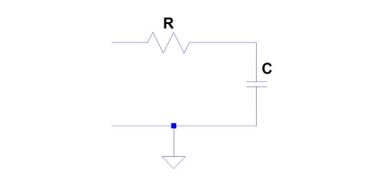
\includegraphics[width = 4in]{./Figures/filter.jpg}
	\rule{35em}{0.5pt}
	\caption{Low pass RC filter}
\end{figure}